\documentclass[titlepage = firstcover]{scrartcl}
\usepackage[aux]{rerunfilecheck}
\usepackage{fontspec}
\usepackage[main=ngerman, english, french]{babel}

% mehr Pakete hier
\usepackage{expl3}
\usepackage{xparse}

%Mathematik------------------------------------------------------
\usepackage{amsmath}   % unverzichtbare Mathe-Befehle
\usepackage{amssymb}   % viele Mathe-Symbole
\usepackage{mathtools} % Erweiterungen für amsmath
\usepackage[
  math-style=ISO,    % \
  bold-style=ISO,    % |
  sans-style=italic, % | ISO-Standard folgen
  nabla=upright,     % |
  partial=upright,   % /
]{unicode-math}% "Does exactly what it says on the tin."
\usepackage[section, below]{placeins}

% Laden von OTF-Mathefonts
% Ermöglich Unicode Eingabe von Zeichen: α statt \alpha

\setmathfont{Latin Modern Math}
%\setmathfont{Tex Gyre Pagella Math} % alternativ zu Latin Modern Math
\setmathfont{XITS Math}[range={scr, bfscr}]
\setmathfont{XITS Math}[range={cal, bfcal}, StylisticSet=1]

\AtBeginDocument{ % wird bei \begin{document}
  % werden sonst wieder von unicode-math überschrieben
  \RenewDocumentCommand \Re {} {\operatorname{Re}}
  \RenewDocumentCommand \Im {} {\operatorname{Im}}
}
\usepackage{mleftright}
\setlength{\delimitershortfall}{-1sp}

%Sprache----------------------------------------------------------
\usepackage{microtype}
\usepackage{xfrac}
\usepackage[autostyle]{csquotes}    % babel
\usepackage[unicode, pdfusetitle]{hyperref}
\usepackage{bookmark}
\usepackage[shortcuts]{extdash}
%Einstellungen hier, z.B. Fonts
\usepackage{booktabs} % Tabellen


\title{Röntgenabsorption}
\author{
  Lasse Sternemann\\
  \href{mailto:lasse.sternemann@udo.edu}{lasse.sternemann@udo.edu}
}
\date{Bearbeitet am 10.05.2020}

\begin{document}
    \maketitle
    \newpage
    \tableofcontents
    \newpage

    \section{Zielsetzung}
        Über die Messung von Absorptionsspektren von Atomen sollen die Übergangsenergien der Elektronen aus der K-Schale bestimmt werden.



    \section{Theoretische Grundlagen}
        \subsection{Röntgenstrahlung}
            Das Röntgenspektrum besteht immer aus einem kontinuierlichem Bremsspektrum und einer Mehrzahl an charakteristischen Strahlungspeaks, die sich mit dem Bremsspektrum überlagern.
            Dieses Spektrum kann mit einer Röntgenröhre erzeugt werden. Sie besteht aus einer Glühkathode, aus der Elektronen über eine Heizspannung ausgelöst werden. Zwischen der Glühkathode und einer
            gegenüber befestigten Anode liegt eine Beschleunigungsspannung an, sodass das resultierende elektrische Feld die Elektronen auf die Anode zubeschleunigt. Die beim Auftreffen auf die Anode 
            entstehenden Strahlungsarten lassen sich über zwei Entstehungsmechanismen erklären.

            \FloatBarrier

            \begin{figure}[h]
              \centering
              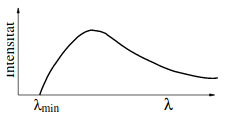
\includegraphics{Brems.png}
              \caption{In der Abbildung ist ein Bremsspektrum schematisch skizziert. Die kleinste Wellenlänge $\lambda$ entspricht der Energie der schnellsten Elektronen. [1]}
              \label{fig:SkizzeBrems}
            \end{figure}

            \FloatBarrier

            \subsubsection{Bremsspektrum}
                Das kontinuierliche Bremspektrum entsteht, wenn die beschleunigten Elektronen durch das Coulumb-Feld der Atome des Anodenmaterials abgebremst. Dies entspricht einer negativen 
                Beschleunigung und die dabei verlorene kinetische Energie des Elektrons wird in Form von Strahlung abgegeben. Die dabei entstehende Energie mit der höchsten Energie, bzw. geringsten 
                Wellenlänge, entspringt den Elektronen, die maximal beschleunigt wurden, also die gesamte Energie des E-Felds aufgenommen haben und beim Abbremsen ihre Energie komplett verlieren. 
                Die zugehörige Energie lässt sich demnach über folgende Formel berechnen:

                \begin{equation*}
                    \lambda = \frac{hc}{\Delta E} \qquad \longrightarrow \qquad \lambda_{\text{Grenz}} = \frac{hc}{U_{\text{Beschl}}\cdot e_0}
                \end{equation*}
                \noindent
            
            \subsubsection{Charakteristische Strahlung}
                Die deutlich erkennbaren Peaks im Röntgenspektrum sind von dem Anodenmaterial der Röntgenröhre abhängig und werden daher als charakteristische Strahlung bezeichnet. Sie entstehen, wenn
                ein beschleunigtes Elektron ein Elektron eines Atoms des Anodenmaterials aus dessen Schale haut. Das ionisierte Atom wird nun in den Grundzustand zurückgesetzt, wenn ein Elektron 
                aus einer höher energetischen Schale hinab an den freigewordenen Schalenplatz springt. Die aus der Potentialdifferenz überschüssige Energie, wird als Röntgenquant mit der
                Wellenlänge \ref{eqn:char} abgegeben und es entstehen scharfe Peaks:
                
                \begin{equation}
                    \lambda_{\text{char}} = \frac{E_{\text{m}}-E_{\text{n}}}{hc}
                    \label{eqn:char}
                \end{equation}
                
                \noindent
                Die aus der Potentialdifferenz frei werdende Energie hängt dabei von den Schalen ab aus der das Elektron herausgelöst und aus der das neue Elektron hinabsteigt. Die Schalenenergien 
                werden in Formel \ref{eqn:char} durch die Indizes "n" und "m" differenziert. Die verschiedenen charakteristischen Peaks ergeben sich daraus, dass der beschriebene Prozess zwischen
                allen Schalen ($K, L, M$) auftreten kann. So werden die Peaks bezüglich der Schale mit der freien Elektronstelle, der Großbuchstabe, und der Schale aus der das neue Elektron kommt,
                der griechische Indize, bezeichnet. Wenn ein Elektron aus der L-Schale, um eine Schale auf die K-Schale fällt, wird der zueghörige Peak als $K_{\alpha}$ bezeichnet. Bei einem Sprung
                um zwei Schalen lautet der Indize $\beta$ und bei drei Schalen $\gamma$. Um aus Formel \ref{eqn:char} die Energie eines Sprunges zu berechnen wird die potentielle Energie in den
                Schalen wie folgt berechnet:

                \begin{equation}
                  E_n = -R_{\infty} \cdot z_{\text{eff}}^2 \cdot \frac{1}{n^2} \qquad \text{Rydbergenergie}: \, R_{\infty}=13,6 \, eV
                  \label{eqn:Schalenenergie}
                \end{equation}
                
                \noindent
                Dabei wird berücksichtigt, dass die Schalenelektronen sich auch gegenseitig abstoßen und so teils vom Coulomb-Feld abgeschirmt werden. Die verringerte Wirkung des Coulomb-Feldes
                wird durch die effektive Kernladungszahl beschrieben, die sich aus der Differenz der grundsätzlichen Kernladungszahl und der Abschirmkonstante $\sigma$ ergibt:
                
                \begin{equation*}
                  z_{\text{eff}} = Z - \sigma
                \end{equation*}
                
                \noindent
                Nun kann durch Einsetzen von \ref{eqn:Schalenenergie} in Gleichung \ref{eqn:char} die Energie einer Übergangslinie aus der Abschirmkonstante der einzelnen Elektronen, der 
                Energieniveaus der beteiligten Schalen und der Kernladungszahl des Elements berechnet werden.
                
                \begin{equation}
                  E_{\text{Endschale}_{\text{m-n}}} = R_{\infty} \cdot (Z - \sigma_n)^2 \cdot \frac{1}{n^2} - R_{\infty} \cdot (Z - \sigma_m)^2 \cdot \frac{1}{m^2}
                  \label{eqn:Energiedifferenz} 
                \end{equation}
                
                \noindent
                Entgegen Gleichung \ref{eqn:Energiedifferenz} haben nicht alle zugehörigen Übergänge genau diese Energie. Dies liegt daran, dass nicht alle Elektronen einer Schale genau dieselbe
                potentielle Energie haben. Daher bestehen die charakteristischen Peaks bei genauerer Betrachtung aus mehreren kleinen, in einer Feinstruktur angeordneten Peaks, die jedoch meist zu 
                einem zusammengefasst werden.

        \subsection{Absorptionsspektrum}
            Wenn die Röntgenstrahlung auf eine Schicht trifft, wird sie teilweise absorbiert. Dies geschieht durch das Auftreten des Photo-Effekts und der Compton-Streuung, wenn die Röntgenquanten
            auf das Absorbermaterial auftreffen. Wenn die Röntgenquanten sehr energiereich sind (E>1MeV) sind diese beiden Effekte nicht mehr als dominant anzusehen, da ihre Wirkungsquerschnitte 
            sinken und weitere Effekte beeinflussen die Absorption. Der für die Größe der Absorption verantwortliche Absorptionskoeffizient sinkt bei steigender Energie. Eine Ausnahme bilden die 
            Energien, die der Bindungsenergie eines Elektrons der nächsthöheren Schale entsprechen. Denn wenn diese erreicht ist, können die Röntgenquanten Elektronen aus ihrer Schale auf freie
            Plätze in eben jener nächsthöheren Schale anheben. Dies geschieht natürlich bei mehreren Energien, da es auch mehrere Schalen gibt. Die für diese Anregungen notwendige Frequenz
            der Röntgenstrahlung berechnet sich wie folgt:

            \begin{equation}
              h \cdot \nu_{\text{abs}} = E_n - E_{\infty}
            \end{equation}
            
            \noindent
            Diese Frequenzen liegen nun an den Absorptionskanten und können auch in die zugehörige Energie umgerechnet werden. Auch hier können z.B bei der L-Kante aufgrund der Feinstruktur mehrere
            Kanten beobachtet werden. Die zu diesen Kanten gehörenden $E_{n,j}$ hängen neben dem Energieniveau $n$ und der effektiven Kernladungszahl nun auch von dem Spin $j$ der einzelnen Elektronen
            auf der Schale und der Sommerfeldschen Feinstrukturkonstante $\alpha$ ab. Diese Energie berechnet sich über Formel \ref{eqn:Enj}.

            \begin{equation}
              E_{n,j} = -R_{\infty} \cdot \left(z_{\text{eff, 1}}^2 \cdot \frac{1}{n^2} + \alpha ^2 z_{\text{eff, 2}}^4 \cdot \frac{1}{n^3} \cdot \left(\frac{1}{j+\frac{1}{2}} - \frac{3}{4n}\right)\right), \qquad z_{\text{eff, n}} = (Z-\sigma_n)
              \noindent \label{eqn:Enj}
            \end{equation}
            
            \noindent
            Aus diesen Gleichungen entspringt die Sommerfeldsche Feinstrukturformel , die die Abschirmkonstante eines Elektrons aus der K-Schale wie folgt berechnet:

            \begin{equation}
              \sigma_{\text{k}} = Z - \sqrt{\frac{E_{\text{K}}}{R_{\infty}} - \frac{\alpha ^2 Z^4}{4}}
              \label{eqn:sigmak}
            \end{equation}
            
            \noindent
            Die  restlichen Abschirmkonstanten einer Schale lassen sich bei Kenntnis der Absorptionskantenenrgie $E_{\text{Endschale}_{\text{m-n}}}$ und von $\sigma_1$, z.B. aus Gleichung 
            \ref{eqn:sigmak} auch durch Umstellen von Gleichung \ref{eqn:Schalenenergie} nach dem gewünschten $\sigma$ bestimmen. So lassen sich $\sigma_{1,2,3}$ der K-Schale nach diesem
            Prinzip mit folgenden drei Formeln berechnen:
            
            \begin{align}
              \sigma_1 &= Z - \sqrt{\frac{E_{\text{k, abs}}}{R_{\infty}}} \\
              \sigma_2 &= Z - \sqrt{4 \cdot \left(Z - \sigma_1\right)^2 - \frac{4 \cdot E_{\text{k}_{\alpha}}}{R_{\infty}}} \\
              \sigma_3 &= Z - \sqrt{9 \cdot \left(Z - \sigma_1\right)^2 - \frac{9 \cdot E_{\text{k}_{\beta}}}{R_{\infty}}} 
              \label{eqn:Cusigmas}
            \end{align}
            \noindent

            \FloatBarrier

            \begin{figure}[h]
              \centering
              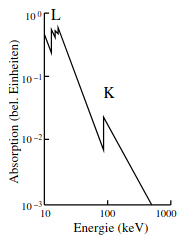
\includegraphics{Kanten.png}
              \caption{In der Abbildung ist ein Absorptionsspektrum dargestellt. Die Sprünge an den Absorptionskanten der L- und K-Schale sind deutlich zu erkennen.[1]}
              \label{fig:SkizzeBragg}
            \end{figure}

            \FloatBarrier



        \subsection{Bragg-Reflexion}
            Bei der Bragg-Reflexion fällt Strahlung auf ein Material mit einer Oberflächengitterstruktur. Wenn Strahlung einer gewissen Wellenlänge auf diese Gitterstruktur auftrifft, wird sie 
            an einem Atom in der Gitterstruktur gebeugt und interferiert daraufhin mit sich selbst. Dabei kommt es beim Bragg-Winkel $\theta$ zu konstruktiver Interferenz. Der Bragg-Winkel hängt
            neben der Wellenlänge der einfallenden Strahlung auch von der Gitterkonstante des Materials $d$ und der Anzahl der Schichten an denen das Licht gebeugt wird $n$ ab. Er lässt sich
            durch Umstellen von Formel berechnen. Da der Bragg-Winkel von der Wellenlänge abhängt, kann man bei konstantem Material Da sie die maximale Inensität beiDa sie die maximale Inensität beibei verschiedenen Winkeln verschiedene Wellenlängen eines 
            einfallenden Spektrums beobachten.

            \begin{equation}
              2d\sin(\theta) = n\lambda \qquad \longrightarrow \qquad \theta = \arcsin(\frac{n\lambda}{2d})
              \label{eqn:Bragg}
            \end{equation}

            \noindent
            Über die Energie eines Quants kann Formel \ref{eqn:Bragg} auch genutzt werden, um die Energie der Strahlung in Abhängigkeit vom Bragg-Winkel zu berechnen.
            
            \begin{equation}
              E = \frac{hc}{\lambda} \qquad \longrightarrow \qquad E = \frac{hcn}{2\cdot d \cdot \sin(\theta)}
              \label{eqn:Energie}
            \end{equation}

            \FloatBarrier

            \begin{figure}[h]
              \centering
              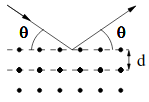
\includegraphics{skizzebragg.png}
              \caption{In der Abbildung ist die Bragg-Reflexion skizziert. Der Winkel $\theta$ ist der Bragg-Winkel und d die Gitterkonstante.[1]}
              \label{fig:SkizzeBragg}
            \end{figure}

            \FloatBarrier


    \section{Durchführung}

    \FloatBarrier

    \begin{figure}[h]
      \centering
      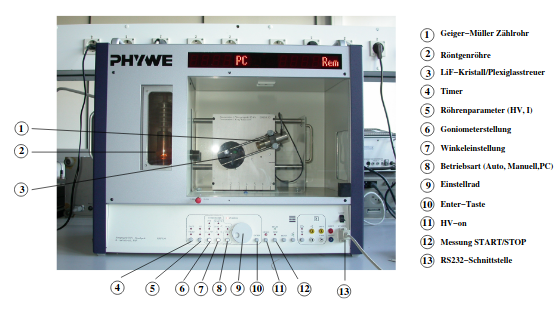
\includegraphics{Aufbau.png}
      \caption{In der Abbildung ist der Gesamtaufbau des Versuches abgebildet. Die einzelnen Komponenten werden zudem benannt.[1]}
      \label{fig:Aufbau}
    \end{figure}

    \FloatBarrier

            
        \subsection{Röntgenstrahlung}
          Um den Versuch durchführen zu können wird zunächst Röntgenstrahlung erzeugt. Dies geschieht wie in Abschnitt (ref) beschrieben in einer Röntgenröhre, die die Elektronen bei einem Emissionsstrom
          von 1mA und einer Beschleunigungsspannung 35kV auf eine Kupferanode beschleunigt. 

        \subsection{Bragg-Bedingung}
          Zunächst soll die Bragg-Bedingung, die eine Aussage über den Winkel des Intensitätsmaximum der reflektieren Strahlung trifft, überprüft werden. Dafür wird ein LiF-Kristall in einem 
          Bragg-Winkel $\theta$ von 14° in den Röntgenstrahl gestellt. Das Intensitätmaxium der reflektierten Röntgenstrahlung wird ebenfalls beim Bragg-Winkel relativ zum LiF-Kristall erwartet. 
          Das Intensitätmaxium wird demnach beim doppelten Winkel $2\theta$ zum Strahl erwartet und daher ein Messbereich von 26° bis 30° gewählt. Ein Geiger-Müller-Zählrohr misst
          für diesen Bereich die Intensität der reflektieren Strahlung in 0,1°-Schritten und über eine Integrationszeit von 5 Sekunden.

        \subsection{Röntgenspektrum}
          Um das Röntgenspektrum der Röntgenröhre mit Kupferanode zu analysieren, wird die Bragg-Bedingung verwendet. Das Geiger-Müller-Zählrohr misst dazu in einem Winkelbereich von 4° bis 26°, was
          dem doppelten Anstellwinkel des LiF-Kristalls zum Röntgenstrahl entspricht, in Schritten von 0,1° und einer Integrationszeit von 5 Sekunden die Intensität der vom LiF-Kristall reflektierten 
          Röntgenstrahlung. Über die Bragg-Bedingung kann jedem Bragg-Winkel eine Wellenlänge zugeordnet werden, sodas nach Abschluss der Messung das Spektrum in Abhängigkeit vom Bragg-Winkel oder der
          Wellenlänge dargestellt werden kann.


        \subsection{Absorptionsspektren}
          Zur Messung von Absorptionsspektren muss zunächst ein Absorber zwischen LiF-Kristall und Geiger-Müller-Zählrohr platziert werden. Nun wird der Winkel des Geiger-Müller-Zählrohrs in 
          0,1°-Schritten über einen für das Material geeigneten Bereich varriert und dabei das Absorptionsspektrum gemessen. Es werden füt Zink, Gallium, Brom, Rubidium, Strontium und Zirkonium
          die zugehörigen Absorptionsspektren gemessen.
          

    
    \section{Auswertung}
        
        Für weitere Rechnungen werden zunächst Elemtareigenschaften aus der Literatur gesucht und berechnet. Die $\sigma_k$s werden dabei aus $E_k^{\text{Lit}}$, der Rydbergenergie $R_{\infty}$, der 
        Ordnungszahl Z und der Sommerfeldschen Feinstrukturkonstante $\alpha$ über Formel \ref{eqn:sigmak} berechnet, die Winkel $\theta_k^{\text{Lit}}$ aus $E_k^{\text{Lit}}$ und der Gitterkonstante d, nach
        Umstellen von Gleichung \ref{eqn:Energie} nach $\theta$ bei n=1.
        
        \begin{equation*}
          \theta_k^{\text{Lit}} = \arcsin\left(\frac{hc}{2 \cdot 201,4 \cdot 10^{-12} \text{m} \cdot E_k^{\text{Lit}}}\right)
        \end{equation*}
        
        \noindent
        So lässt sich unter Recherche von $E_k^{\text{Lit}}$ und Z die folgende Tabelle komplett ausfüllen.
        \FloatBarrier
        \begin{table}[h]
          \centering
          \caption{In der Tabelle sind Literaturwerte von Eigenschaften der im Experiment verwendeten Elemente dragestellt. Sie werden teils auseinander errechnet.}
          \label{tab:Elemente}
        
          \begin{tabular}{c c c c c}
            \toprule
            {Material}  & {Ordnungszahl Z} & {$E_k^{\text{Lit}}$ [eV]} & {$\theta_k^{\text{Lit}}$ [°]} & {$\sigma_k$} \\ 
            \midrule
            Cu	                &   29           &  8980          &  20,05     &    3,31   \\
            Zn	                &   30           &  9650          &  18,60     &    3,57   \\
            Ga	                &   31           &  10370         &  17,27     &    3,62   \\
            Br	                &   35           &  13470         &  13,21     &    3,85   \\
            Rb	                &   37           &  15200         &  11,68     &    3,95   \\
            Sr	                &   38           &  16100         &  11,02     &    4,01   \\
            Zr	                &   40           &  17990         &  9,85      &    4,11   \\
            \bottomrule
          \end{tabular}
        \end{table}
  
        \FloatBarrier
        
        \subsection{Überprüfung der Bragg-Bedingung}
            Um die Bragg-Bedingung zu überprüfen wird der LiF-Kristall in einem Winkel $\theta$ von 14° in den Röntgenstrahl gestellt. Aus Skizze \ref{fig:SkizzeBragg} geht hervor, dass das 
            Intensitätsmaximum der reflektierten Strahlung bei einem Winkel von $2\theta$, also 28°, zum Strahl zu finden sein sollte.
            \FloatBarrier
            \begin{figure}[h]
              \centering
              \caption{In dem Graphen ist die Impulsrate der am LiF-Kristall reflektierten Röntgenstrahlung in Imp/s gegen den Messwinkel des Geiger-Müller-Zählrohrs relativ zum Röntgenstrahl aufgetragen. Das Intensitätsmaximum liegt bei 28,2°.}
              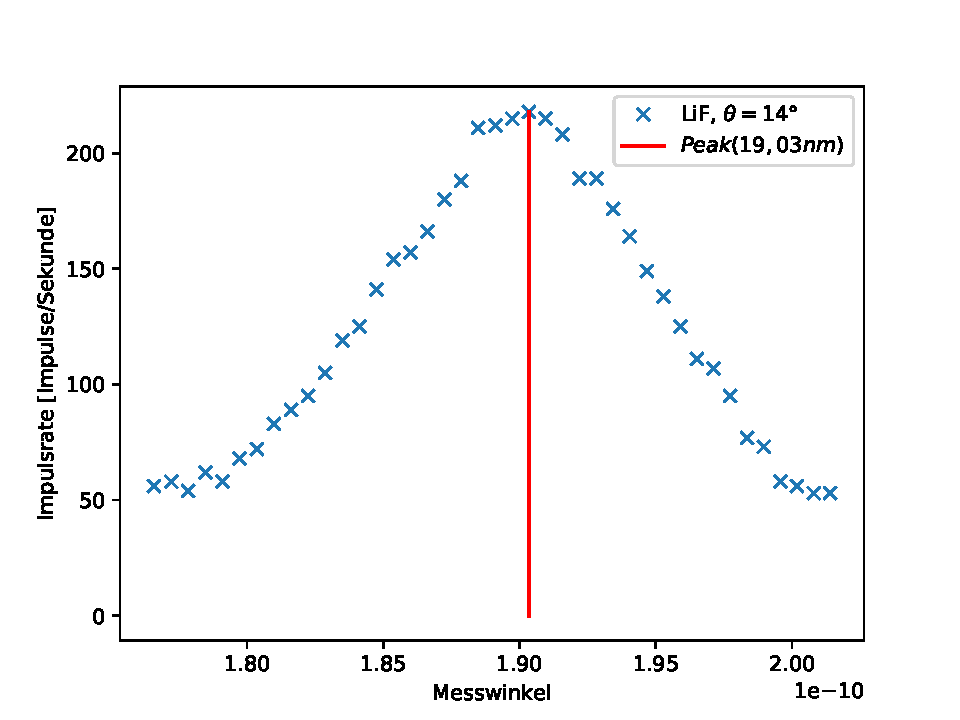
\includegraphics{Bragg.pdf}
              \label{fig:bragggraph}
            \end{figure}
            \FloatBarrier  

            \noindent
            Die Auswertung der in Grafik \ref{fig:graphbragg} dargestellten Messwerte über die Scipy-Funktion findPeaks liefert das Intensitätsmaximum bei einem Winkel von $(28,2 \pm 0,1)°$. 


        \subsection{Emissionspektrum}
            Zunächst werden die gesamten Messdaten der Messung zur Intensität in Abhängigkeit vom Bragg-Winkel in einer Grafik
            \FloatBarrier
            \begin{figure}[h]
              \centering
              \caption{In dem Graphen ist der gesamte Bereich des aufgenommen Röntgenspektrums der Kupferröntgenröhre, in Form der Impulsrate in Imp/s in Abhängigkeit vom Bragg-Winkel aufgetragen. Neben dem kontinuierlichen Bremsspektrum sind auch die $K_{\alpha}-$ und $K_{\beta}-$ Peaks deutlich zu erkennen.}
              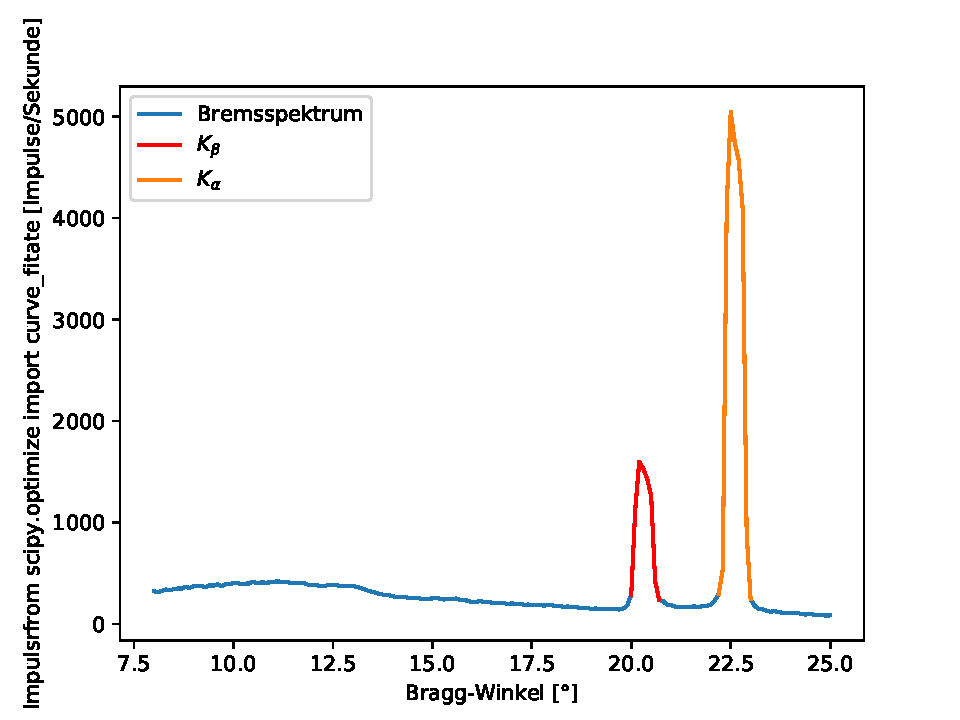
\includegraphics{Spektrum_Cu.pdf}
              \label{fig:spektrum}
            \end{figure}
            \FloatBarrier
            \noindent
            Zur genaueren Betrachtung der charakteristischen Strahlung wird zudem ein Detailspektrum der $K_{\alpha}-$ und $K_{\beta}-$ Peaks angefertigt. In diesem Detailspektrum wird der durch die 
            Bremstrahlung erzeugte Untegrund über folgende Geradengleichung abgezogen.

            \begin{equation*}
              y = -35,10 \cdot x + 795,04
            \end{equation*}

            \noindent
            So ergibt sich folgende Grafik, die nur noch die Peaks enthält.
            \FloatBarrier
            \begin{figure}[h]
              \centering
              \caption{In dem Graphen sind nun nur noch die charakteristischen Peaks des Röntgenspektrums der Kupferröntgenröhre, in Form der Impulsrate in Imp/s in Abhängigkeit vom Bragg-Winkel aufgetragen, da der Untegrund des Bremsspektrums abgezogen wurde. Die Halbwertsbreite des $K_{\beta}-$ Peaks (links) und des $K_{\alpha}-$ Peaks (rechts) sind durch die Grünen Boxen gekennzeichnet.}
              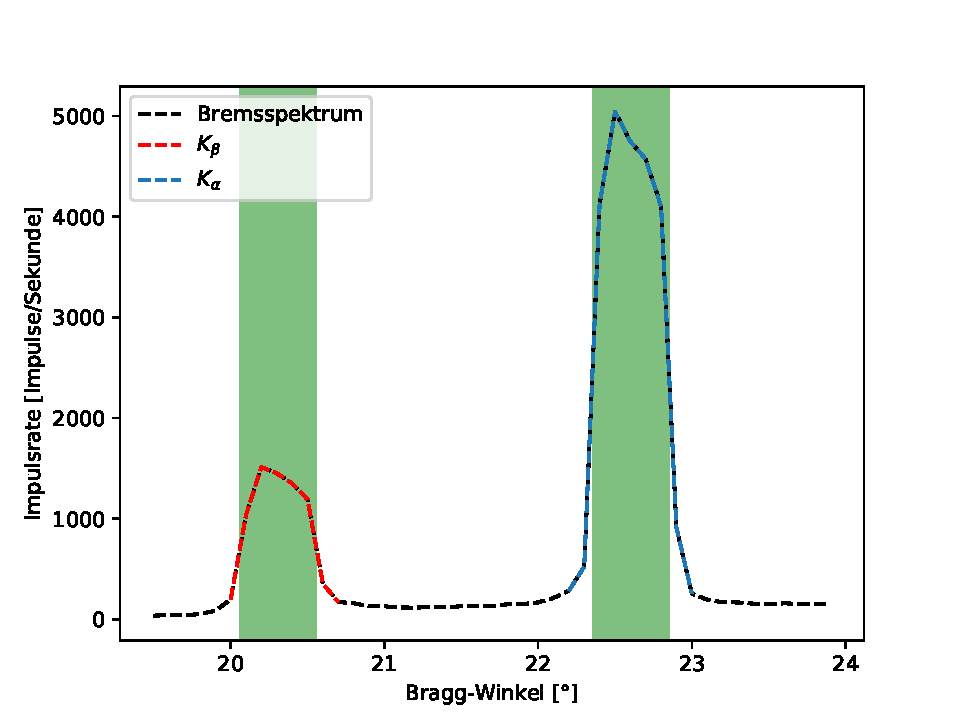
\includegraphics{Peaks_Cu.pdf}
              \label{fig:graphpeak}
            \end{figure}
            \FloatBarrier
            \noindent
            Die Halbwertsbreiten der Peaks des angepassten Spektrums wird über einen Spline berechnet und ist in Grafik als grüne Box eingezeichnet. Über Formel \ref{eqn:Energie} mit n=1 in die 
            Energie umgerechnet, ergeben sie sich als 

            \begin{equation*}
              \Delta E_{\beta} = 210 \, \text{eV} \qquad \text{und} \qquad \Delta E_{\alpha} = 170 \, \text{eV}
              \label{eqn:Breiten}
            \end{equation*}
            
            \noindent
            Aus diesen Energien und den Energien der charakteristischen Peaks, die aus den Winkeln

            \begin{equation*}
              \theta_{\beta} = 20,1 \pm 0,1     \qquad \theta_{\alpha} = 22,4 \pm 0,1
            \end{equation*}

            \noindent
            über Formel \ref{eqn:Energie}, bei n=1, und deren Fehler über folgende Formel berechnet wird:

            \begin{equation*}
              \Delta E = \frac{hcn}{2d} \cdot \frac{2 \cdot \cos(\theta)}{\cos(2\theta)-1}
            \end{equation*}
            
            \begin{equation}
              E_{\beta} = 8910 \pm 40 \, \text{eV} \qquad \text{und} \qquad E_{\alpha} = 8043 \pm 34\, \text{eV}
              \label{eqn:Energiepeak}
            \end{equation}
            
            \noindent
            werden die Auflösungen der Peaks berechnet:

            \begin{equation}
              \text{Auflösung} = \frac{E_{\text{Peak}}}{\Delta E_{\text{Peak}}} \qquad \longrightarrow \qquad \text{Auflösung}_{\beta} = 42,55 \pm 0,20 , \qquad \text{Auflösung}_{\alpha} = 47,85 \pm 0,20
            \end{equation}
            
            \noindent
            Zuletzt werden aus den Formeln \ref{eqn:Cusigmas} die Abschirmkonstanten $\sigma_1, \sigma_2$ und $\sigma_3$ des Kupferatoms bestimmt, dazu werden die bestimmten Energien der Peaks
            \ref{eqn:Energiepeak} und das $E_{\text{k, abs}}$ aus der Eigenschaftentabelle der Elemente verwendet. Da $\sigma_1$ über Literaturwerte berechnet wird, bleibt es fehlerfrei. Die Fehler zu
            $\sigma_2$ und $\sigma_3$ ergeb sich wiefolgt:

            \begin{align*}
              \Delta \sigma_2 = \frac{2}{R_{\infty} \cdot \sqrt{4 \cdot \left(Z - \sigma_1 \right)^2 - \frac{4E_K}{R_{\infty}}}} \cdot \Delta E_K \\
              \Delta \sigma_3 = \frac{9}{2 \cdot R_{\infty} \cdot \sqrt{9 \cdot \left(Z - \sigma_1 \right)^2 - \frac{9E_K}{R_{\infty}}}} \cdot \Delta E_K
            \end{align*}
            
            \begin{align*}
              \sigma_1 &= 3,31 \\
              \sigma_2 &= 12,41 \pm 0,30 \\
              \sigma_3 &= 22,40 \pm 2,1
            \end{align*}
            \noindent

          
          \subsection{Absorptionsspektren}
            Die gemessenen Absorptionsspektren der Absorbermaterialien Zink \ref{fig:Zink}, Gallium \ref{fig:Gallium}, Brom \ref{fig:Brom}, Rubidium \ref{fig:Rubidium}, Strontium \ref{fig:Strontium}
            und Zirkonium \ref{fig:Zirkonium} werden dargestellt, indem die Impulsrate der absorbierten Strahlung gegen den zugehörigen Bragg-Winkel aufgetragen wird. 
            Aus diesen Absorptionsspektren, die die K-Kante enthalten, werden die zur K-Kante gehörigen Energien bestimmt. Um zunächst die Mitte der gemessenen Kante zu bestimmen, wird 
            der Intensitätswert der Mitte zwischen dem Maximum und Minimum der Kante berechnet, indem eine Gerade zwischen den Punkten gelegt wird und die Intensität in der Mitte dieser berechnet
            wird.
            
            \begin{equation}
              I_{\text{K}} = I_{\text{K}}^{\text{min}} + \frac{I_{\text{K}}^{\text{min}} + I_{\text{K}}^{\text{max}}}{2}
              \label{eqn:EFehler}
            \end{equation}

            \noindent
            Daraufhin wird der dieser Intensität zugehörige Wert aus dem Datensatz der Intensitäten und zugehörigen Winkel berechnet. Aus diesem Winkel wird die, der Kante zugehörige, Energie über 
            Formel \ref{eqn:Energie} und der Fehler wieder über \ref{eqn:EFehler} berechnet. Aus diesen Energien wiederum werden die den K-Schalen zugehörigen Abschirmkonstanten $\sigma_{\text{k}}$ 
            über Formel \ref{eqn:sigmak} berechnet. Der zugehörige Fehler berechnet sich über folgende Gleichung.
            \begin{equation*}
              \Delta \sigma_k = \frac{1}{2 \cdot R_{\infty}\cdot \sqrt{\frac{E_K}{R_{\infty}} - \frac{\alpha^2 \cdot Z^4}{4}}}
            \end{equation*}
            \noindent
            Die Datensätze der Absorber Zinn, Gallium, Brom, Rubidium, Strontium und Zirkonium ergeben folgende Werte. 
            \FloatBarrier
            \begin{table}[h]
              \centering
              \caption{In der Tabelle sind die abgelesenen Maxima und Minima der Intensität vor $I_{\text{K}}^{\text{min}}$ und nach $I_{\text{K}}^{\text{max}}$ der Kante sowie die daraus bestimmte mittlere Intensität der Kante dargestellt. Der dieser Intensität zugehörige Winkel $\theta$, sowie die daraus berechnete Energie $E_{\text{K}}$ und Abschirmkonstante $\sigma_k$ sind ebenfalls für alle Materialien eingetragen.}
              \label{tab:Absorption}
            
              \begin{tabular}{c c c c c c c}
                \toprule
                {Material}  & {$I_{\text{K}}^{\text{min}}$ [Imp/s]} & {$I_{\text{K}}^{\text{max}}$ [Imp/s]} & {$I_{\text{K}}$ [Imp/s]} & {$\theta$ [°]} & {$E_{\text{K}} \text{[eV]}$} & {$\sigma_k$} \\ 
                \midrule
                Zn	                &  54              & 102           &    78       &    18,7 $\pm$ 0,1  &   9600 $\pm$ 50   &   3,64 $\pm$ 0,07   \\
                Ga	                &  66              &  122          &    94       &   17,3  $\pm$ 0,1  &   10350$\pm$ 60   &   3,64 $\pm$ 0,08    \\
                Br	                &  9               &  27           &    18       &   13,2  $\pm$ 0,1  &   13480$\pm$ 100  &   3,84 $\pm$ 0,12  \\
                Rb	                &  12              &  64           &    38       &   11,8  $\pm$ 0,1  &   15050$\pm$ 130  &   4,12 $\pm$ 0,14   \\
                Sr	                &  40              &  196          &    118      &    11,1 $\pm$ 0,1  &   15990$\pm$ 140  &   4,13 $\pm$ 0,15   \\
                Zr	                &  112             &  301          &    206,5    &    10   $\pm$ 0,1  &   17730$\pm$ 180  &   4,38 $\pm$ 0,18   \\
                \bottomrule
              \end{tabular}
            \end{table}
            \FloatBarrier
            \noindent
            Zuletzt wird die Rydbergenergie $R_{\text{inf}}$ mit Hilfe des  Moseley´schen Gesetz bestimmt. Diese besagt, dass die Wurzel der K-Kantenenergie der Elemente gegen die effektive 
            Kernladungszahl des Elements eine Gerade ergeben, deren Steigung die Wurzel der Rydbergenergie ergibt. Dazu werden eben diese Werte per Matplotlib in Grafik \ref{fig:Moseley} 
            aufgetragen und mit der Funktion Curvefit eine lineare Regression angefertigt, die folgende Parameter hat:

            \begin{align*}
              y &= mx + b \\
              m &= (1518,91 \pm 2,03) \cdot 10^{-12} \qquad b = (-831,75 \pm 63,60) \cdot 10^{-12} \\
            \end{align*}

            \noindent
            Aus der Steigung $m$ wird dann die Rydbergenergie $R_{\text{inf}}$ bestimmt:

            \begin{equation*}
              R_{\text{inf}} = m^2 = (14,40 \pm 0,04) \, \text{eV}
            \end{equation*}
            
            \FloatBarrier
            \begin{figure}[h]
              \centering
              \caption{In dem Graphen sind die Wurzeln der K-Kantenenergien gegen die effekktiven Kernladungszahlen der Elemente $(Z-\sigma)$ aufgetragen.}
              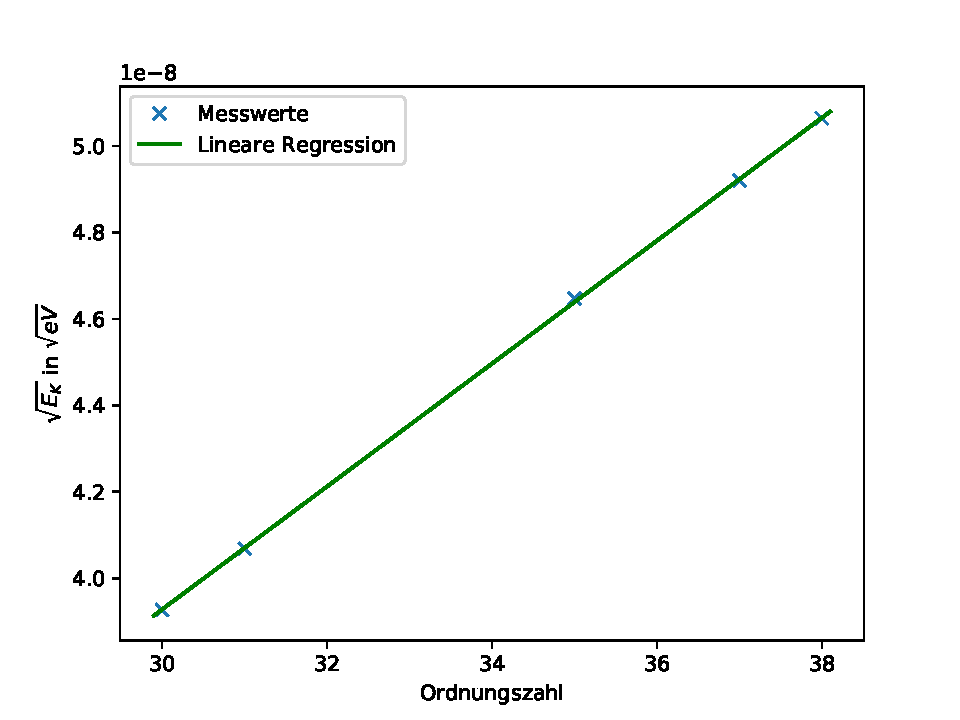
\includegraphics{Moseley.pdf}
              \label{fig:Moseley}
            \end{figure}
            \FloatBarrier


          \section{Diskussion}
            Die zunächst durchgeführte Überprüfung der Bragg-Bedingung hat einen Winkel ergeben, der um 0,2° vom Literaturwert abweicht. Die kleine Abweichung lässt sich womöglich durch Unebenheiten
            in der kristallinen Struktur erklären. Dennoch ist der Wert aussagekräftig genug, um die Theorie zur Lage des Intensitätmaxium bei der Bragg-Reflexion zu bestätigen. Die Literaturenergien 
            der Peaks des charakteristischen Spektrums liegen beide im $1\sigma$-Bereich der Messwerte. Dementsprechend decken sich diese Messwerte mit der Theorie. Auch die Literaturwerte der 
            Abschirmkonstanten $\sigma_1, \sigma_2$ und $\sigma_3$ liegen im $1\sigma$-Bereich der Messwerte, sodass die Messwerte ein gutes Bild der Theorie abbilden.
            Daraufhin wurden die Absorptionskantenenergien der Materialien Zink, Gallium, Brom, Rubidium, Strontium und Zirkonium bestimmt. Während die Energien von Zink, Gallium, Brom und Strontium
            innerhalb der $1\sigma$-Umgebung liegen und somit sehr gut mit den Experimentalwerten übereinstimmen, liegen die Literaturenergien von Rubidium und Zirkonium leicht außerhalb des 
            $1\sigma$-Bereichs. Die Abweichung ist jedoch gering und auch diese Werte können über die Literaturenergien bestätigt werden. Da die Abschirmkonstanten der einzelnen Materialien aus 
            den zuvor bestimmten Absorptionskantenenergien berechnet werden, deckt sich das beobachtete Fehlerbild mit dem der Energien. Die Literaturwerte von Zink, Gallium, Brom und Strontium
            liegen wieder im $1\sigma$-Bereich der Messwerte und die Literaturwerte von Rubidium und Zirkonium wieder knapp außerhalb. Die Abschirmkonstante von Zirkonium liegt am weitesten vom 
            Literaturwert entfernt und ist nur schwer durch diesen zu bestätigen. Die anderen Abschirmkonstanten decken sich alle gute mit den zugehörigen Literaturwerten. Der $1\sigma$-Bereich 
            des zuletzt bestimmten Wert der Rydbergenergie $\text{R}_{\infty}$ enthält nicht den LIteraturwert. Dennoch ist die Messung als erfolgreich zu beschreiben, da der Experimentalwert um
            5,8 \% vom Literaturwert abweicht und so eine gegnügende Genauigkeit besitzt. 







          \begin{table}[h]
            \centering
            \caption{In der Tabelle werden die Messwerte mit den Literaturwerten verglichen. Da lediglich ein Vergleich des Wertes von Nöten ist, werden die Einheiten nicht mit aufgeschrieben und die Exponenten möglichst gekürzt.}
            
            \begin{tabular}{c c c c c c }
                \toprule
                {Messgröße} & {Messwert} & {Literaturwert} & {Messgröße} & {Messwert} & {Literaturwert} \\
                \midrule

                $E_{\text{K}_{\alpha}}$ [eV] & 8043$\pm$34      & 8038  & $\sigma_{\text{K, Zn}}$  & 3,64 $\pm$ 0,07  & 3,57  \\
                $E_{\text{K}_{\beta}}$ [eV]  & 8910$\pm$40       & 8905 & $\sigma_{\text{K, Ga}}$  & 3,64 $\pm$ 0,08  & 3,62  \\
                $\sigma_{\text{K1}}$         & 3,31 $\pm$ 0     & 3,31  & $\sigma_{\text{K, Br}}$  & 3,84 $\pm$ 0,12  & 3,85  \\
                $\sigma_{\text{K2}}$         & 12.41 $\pm$ 0,30 & 12,36 & $\sigma_{\text{K, Rb}}$  & 4,12 $\pm$ 0,14  & 3,95  \\
                $\sigma_{\text{K3}}$         & 22,40 $\pm$ 2,10 & 21,96 & $\sigma_{\text{K, Sr}}$  & 4,13 $\pm$ 0,15  & 4,01  \\
                $E_{\text{K, Zn}}$ [eV]      & 9600 $\pm$ 50    & 9650  & $\sigma_{\text{K, Zr}}$  & 4,38 $\pm$ 0,18  & 4,11  \\
                $E_{\text{K, Ga}}$ [eV]      & 10350 $\pm$ 60   & 10370 & $\text{R}_{\infty}$ [eV] & 14,40 $\pm$ 0,04 & 13,61 \\
                $E_{\text{K, Br}}$ [eV]      & 13480 $\pm$ 100  & 13470 &                          &                  &       \\
                $E_{\text{K, Rb}}$ [eV]      & 15050 $\pm$ 130  & 15200 &                          &                  &       \\
                $E_{\text{K, Sr}}$ [eV]      & 15990 $\pm$ 140  & 16100 &                          &                  &       \\
                $E_{\text{K, Zr}}$ [eV]      & 17730 $\pm$ 180  & 17990 &                          &                  &       \\
                \bottomrule
            \end{tabular}
        \end{table}



            \newpage
            \section{Anhang}
            \FloatBarrier
            \subsection{Wertetabelle - Bragg-Reflexion}
            \begin{table}
              \centering
              \caption{In der Tabelle sind die Wertepaare der Intensität und des Reflexionswinkels bei Bragg-Reflexion an einem Lif-Kristall eingetragen.}

              \begin{tabular} {c c}
                \toprule
                {$\theta$ [°]} & {I [Imp/s]}  \\
                \midrule
                26,0$\pm$ 0,1 & 	56,0    \\
                26,1$\pm$ 0,1 & 	58,0    \\
                26,2$\pm$ 0,1 & 	54,0    \\
                26,3$\pm$ 0,1 & 	62,0    \\
                26,4$\pm$ 0,1 & 	58,0    \\
                26,5$\pm$ 0,1 & 	68,0    \\
                26,6$\pm$ 0,1 & 	72,0    \\
                26,7$\pm$ 0,1 & 	83,0    \\
                26,8$\pm$ 0,1 & 	89,0    \\
                26,9$\pm$ 0,1 & 	95,0    \\
                27,0$\pm$ 0,1 & 	105,0   \\
                27,1$\pm$ 0,1 & 	119,0   \\
                27,2$\pm$ 0,1 & 	125,0   \\
                27,3$\pm$ 0,1 & 	141,0   \\
                27,4$\pm$ 0,1 & 	154,0   \\
                27,5$\pm$ 0,1 & 	157,0   \\
                27,6$\pm$ 0,1 & 	166,0   \\
                27,7$\pm$ 0,1 & 	180,0   \\
                27,8$\pm$ 0,1 & 	188,0   \\
                27,9$\pm$ 0,1 & 	211,0   \\
                28,0$\pm$ 0,1 & 	212,0   \\
                28,1$\pm$ 0,1 & 	215,0   \\
                28,2$\pm$ 0,1 & 	218,0   \\
                28,3$\pm$ 0,1 & 	215,0   \\
                28,4$\pm$ 0,1 & 	208,0   \\
                28,5$\pm$ 0,1 & 	189,0   \\
                28,6$\pm$ 0,1 & 	189,0   \\
                28,7$\pm$ 0,1 & 	176,0   \\
                28,8$\pm$ 0,1 & 	164,0   \\
                28,9$\pm$ 0,1 & 	149,0   \\
                29,0$\pm$ 0,1 & 	138,0   \\
                29,1$\pm$ 0,1 & 	125,0   \\
                29,2$\pm$ 0,1 & 	111,0   \\
                29,3$\pm$ 0,1 & 	107,0   \\
                29,4$\pm$ 0,1 & 	95,0    \\
                29,5$\pm$ 0,1 & 	77,0    \\
                29,6$\pm$ 0,1 & 	73,0    \\
                29,7$\pm$ 0,1 & 	58,0    \\
                29,8$\pm$ 0,1 & 	56,0    \\
                29,9$\pm$ 0,1 & 	53,0    \\
                30,0$\pm$ 0,1 & 	53,0    \\
                \bottomrule  
              \end{tabular}
            \end{table}
            \FloatBarrier

            \newpage
            \subsection{Wertetabelle - Absorptionsspektren}
            In den Tabellen sind die zu den einzelnen Materialien gehörigen Wertepaare zur Messung der Absorptionskanten eingetragen.
            \FloatBarrier
            \begin{table}
              \centering
              \caption{In der Tabelle sind die Wertepaare der Materialien Zink, Gallium und Brom eingetragen.}

              \begin{tabular} {c c c c c c}
                \toprule
                {$\theta_{\text{Zn}}$ [°]} & {$I_{\text{Zn}}$ [Imp/s]} & {$\theta_{\text{Ga}}$ [°]} & {$I_{\text{Ga}}$ [Imp/s]} & {$\theta_{\text{Br}}$ [°]} & {$I_{\text{Br}}$ [Imp/s]} \\
                \midrule
                18,0 $\pm$ 0,1	& 58,0   & 17,0 $\pm$ 0,1  & 66,0   & 12,8$\pm$ 0,1 & 10,0 \\
                18,1 $\pm$ 0,1	& 54,0   & 17,1 $\pm$ 0,1  & 66,0   & 12,9$\pm$ 0,1 & 12,0 \\
                18,2 $\pm$ 0,1	& 55,0   & 17,2 $\pm$ 0,1  & 78,0   & 13,0$\pm$ 0,1 & 9,0  \\
                18,3 $\pm$ 0,1	& 54,0   & 17,3 $\pm$ 0,1  & 88,0   & 13,1$\pm$ 0,1 & 13,0 \\
                18,4 $\pm$ 0,1	& 54,0   & 17,4 $\pm$ 0,1  & 102,0  & 13,2$\pm$ 0,1 & 18,0 \\
                18,5 $\pm$ 0,1	& 55,0   & 17,5 $\pm$ 0,1  & 116,0  & 13,3$\pm$ 0,1 & 21,0 \\
                18,6 $\pm$ 0,1	& 65,0   & 17,6 $\pm$ 0,1  & 121,0  & 13,4$\pm$ 0,1 & 25,0 \\
                18,7 $\pm$ 0,1	& 84,0   & 17,7 $\pm$ 0,1  & 121,0  & 13,5$\pm$ 0,1 & 27,0 \\
                18,8 $\pm$ 0,1	& 91,0   & 17,8 $\pm$ 0,1  & 122,0  & 13,6$\pm$ 0,1 & 27,0 \\
                18,9 $\pm$ 0,1	& 100,0  & 17,9 $\pm$ 0,1  & 122,0  & 13,7$\pm$ 0,1 & 22,0 \\
                19,0 $\pm$ 0,1	& 102,0  & 18,0 $\pm$ 0,1  & 119,0  & 13,8$\pm$ 0,1 & 25,0 \\
                19,1 $\pm$ 0,1	& 100,0  & 18,1 $\pm$ 0,1  & 114,0  & 13,9$\pm$ 0,1 & 21,0 \\
                19,2 $\pm$ 0,1	& 98,0   & 18,2 $\pm$ 0,1  & 110,0  & 14,0$\pm$ 0,1 & 23,0 \\
                19,3 $\pm$ 0,1	& 100,0  & 18,3 $\pm$ 0,1  & 108,0  & 14,1$\pm$ 0,1 & 20,0 \\
                19,4 $\pm$ 0,1	& 95,0   & 18,4 $\pm$ 0,1  & 104,0  & 14,2$\pm$ 0,1 & 21,0 \\
                19,5 $\pm$ 0,1	& 98,0   & 18,5 $\pm$ 0,1  & 110,0  & 14,3$\pm$ 0,1 & 19,0 \\
                              &          & 18,6 $\pm$ 0,1  & 110,0  &               &      \\
                              &          & 18,7 $\pm$ 0,1  & 109,0  &               &      \\
                              &          & 18,8 $\pm$ 0,1  & 99,0   &               &      \\
                              &          & 18,9 $\pm$ 0,1  & 100,0  &               &      \\
                              &          & 19,0 $\pm$ 0,1  & 98,0   &               &      \\
                \bottomrule  
              \end{tabular}
            \end{table}

            \begin{table}
              \centering
              \caption{In der Tabelle sind die Wertepaare der Materialien Rubidium, Strontium und Zirkonium eingetragen.}

              \begin{tabular} {c c c c c c}
                \toprule
                {$\theta_{\text{Rb}}$ [°]} & {$I_{\text{Rb}}$ [Imp/s]} & {$\theta_{\text{Sr}}$ [°]} & {$I_{\text{Sr}}$ [Imp/s]} & {$\theta_{\text{Zr}}$ [°]} & {$I_{\text{Zr}}$ [Imp/s]} \\
                \midrule
                11,2 $\pm$ 0,1	& 11,0   & 10,5 $\pm$ 0,1  & 43,0   &  9,5$\pm$ 0,1 & 112,0 \\
                11,3 $\pm$ 0,1	& 10,0   & 10,6 $\pm$ 0,1  & 41,0   &  9,6$\pm$ 0,1 & 120,0 \\
                11,4 $\pm$ 0,1	& 10,0   & 10,7 $\pm$ 0,1  & 40,0   &  9,7$\pm$ 0,1 & 126,0 \\
                11,5 $\pm$ 0,1	& 12,0   & 10,8 $\pm$ 0,1  & 44,0   &  9,8$\pm$ 0,1 & 147,0 \\
                11,6 $\pm$ 0,1	& 17,0   & 10,9 $\pm$ 0,1  & 50,0   &  9,9$\pm$ 0,1 & 180,0 \\
                11,7 $\pm$ 0,1	& 32,0   & 11,0 $\pm$ 0,1  & 89,0   & 10,0$\pm$ 0,1 & 225,0 \\
                11,8 $\pm$ 0,1	& 39,0   & 11,1 $\pm$ 0,1  & 120,0  & 10,1$\pm$ 0,1 & 266,0 \\
                11,9 $\pm$ 0,1	& 47,0   & 11,2 $\pm$ 0,1  & 152,0  & 10,2$\pm$ 0,1 & 282,0 \\
                12,0 $\pm$ 0,1	& 57,0   & 11,3 $\pm$ 0,1  & 181,0  & 10,3$\pm$ 0,1 & 290,0 \\
                12,1 $\pm$ 0,1	& 64,0   & 11,4 $\pm$ 0,1  & 193,0  & 10,4$\pm$ 0,1 & 301,0 \\
                12,2 $\pm$ 0,1	& 61,0   & 11,5 $\pm$ 0,1  & 181,0  & 10,5$\pm$ 0,1 & 295,0 \\
                12,3 $\pm$ 0,1	& 57,0   & 11,6 $\pm$ 0,1  & 196,0  & 10,6$\pm$ 0,1 & 283,0 \\
                12,4 $\pm$ 0,1	& 54,0   & 11,7 $\pm$ 0,1  & 181,0  & 10,7$\pm$ 0,1 & 296,0 \\
                12,5 $\pm$ 0,1	& 54,0   & 11,8 $\pm$ 0,1  & 173,0  & 10,8$\pm$ 0,1 & 283,0 \\
                              	&        & 11,9 $\pm$ 0,1  & 166,0  & 10,9$\pm$ 0,1 & 286,0 \\
                              	&        & 12,0 $\pm$ 0,1  & 159,0  & 11,0$\pm$ 0,1 & 286,0 \\
                \bottomrule  
              \end{tabular}
            \end{table}
            \FloatBarrier

            \newpage
            \subsection{Absorptionsspektren}
            In den Grafiken sind die Absorptionsspektren der einzelnen Absorbermaterialien dargestellt, wobei die Winkel indirket die Energie der absorbierten Strahlung und die Impulsrate die 
            Intensität der absorbierten Strahlung wiedergibt. Der plötzliche Anstieg in den Graphen markiert dabei die K-Kante.

            \FloatBarrier
            \begin{figure}[h]
              \centering
              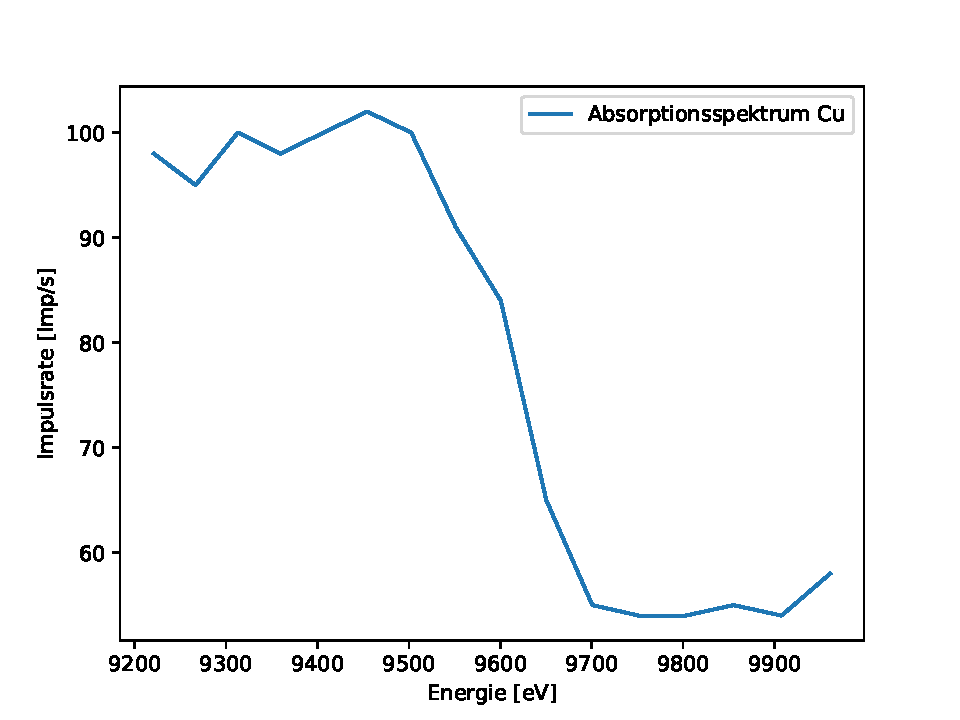
\includegraphics{Zink.pdf}
              \caption{In der Abbildung ist das Absorptionsspektrum des Zink-Absorbers aufgetragen.}
              \label{fig:Zink}
            \end{figure}

            \begin{figure}[h]
              \centering
              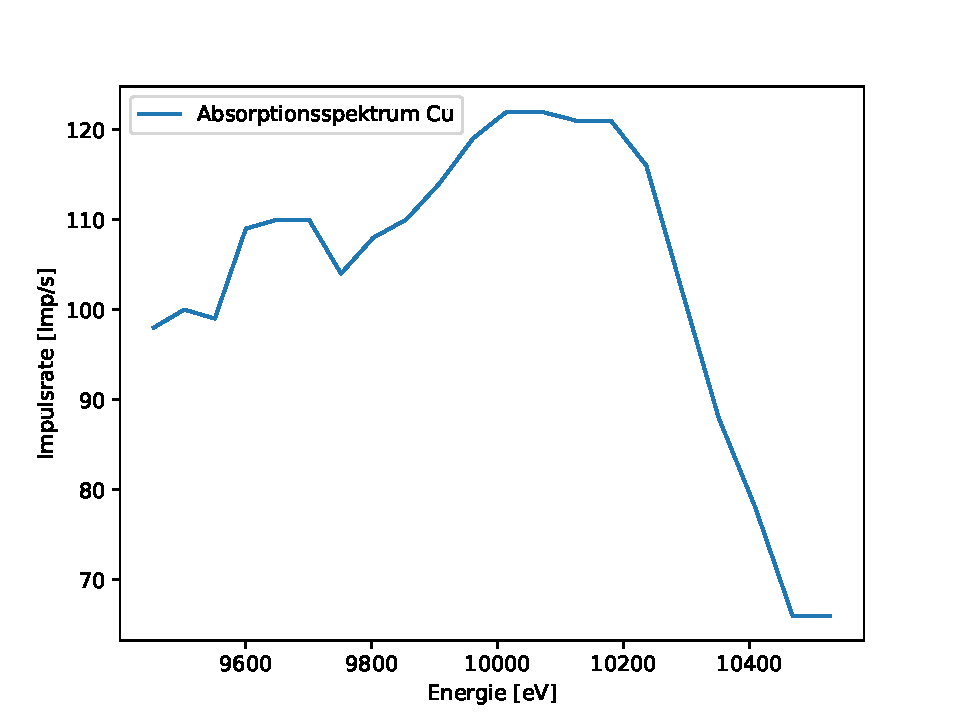
\includegraphics{Gallium.pdf}
              \caption{In der Abbildung ist das Absorptionsspektrum des Gallium-Absorbers aufgetragen.}
              \label{fig:Gallium}
            \end{figure}

            \begin{figure}[h]
              \centering
              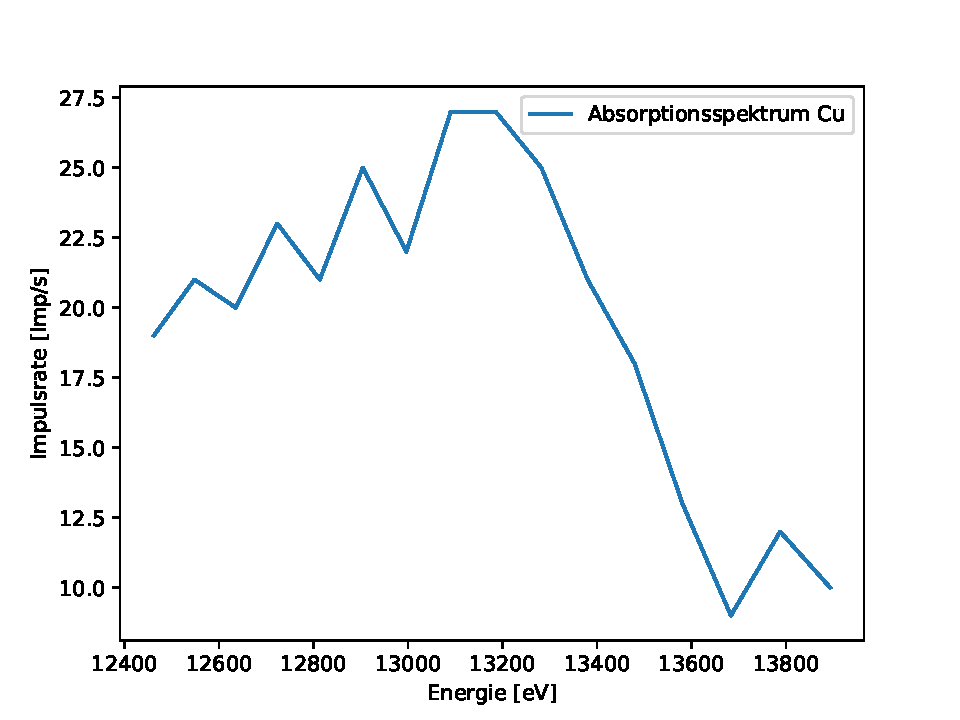
\includegraphics{Brom.pdf}
              \caption{In der Abbildung ist das Absorptionsspektrum des Brom-Absorbers aufgetragen.}
              \label{fig:Brom}
            \end{figure}

            \begin{figure}[h]
              \centering
              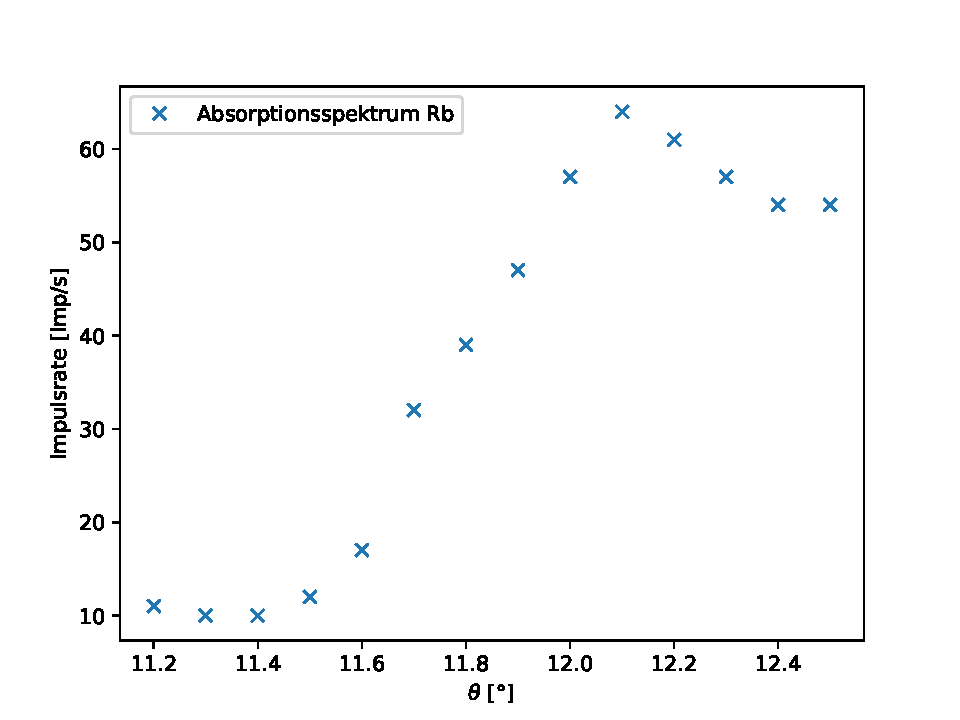
\includegraphics{Rubidium.pdf}
              \caption{In der Abbildung ist das Absorptionsspektrum des Rubidium-Absorbers aufgetragen.}
              \label{fig:Rubidium}
            \end{figure}

            \begin{figure}[h]
              \centering
              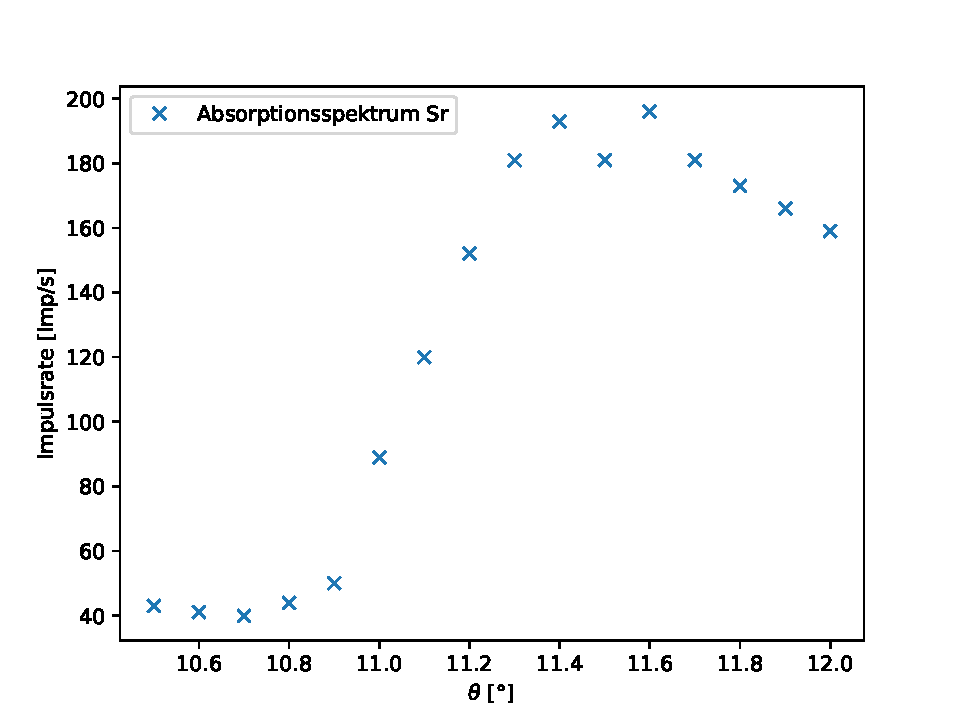
\includegraphics{Strontium.pdf}
              \caption{In der Abbildung ist das Absorptionsspektrum des Strontium-Absorbers aufgetragen.}
              \label{fig:Strontium}
            \end{figure}

            \begin{figure}[h]
              \centering
              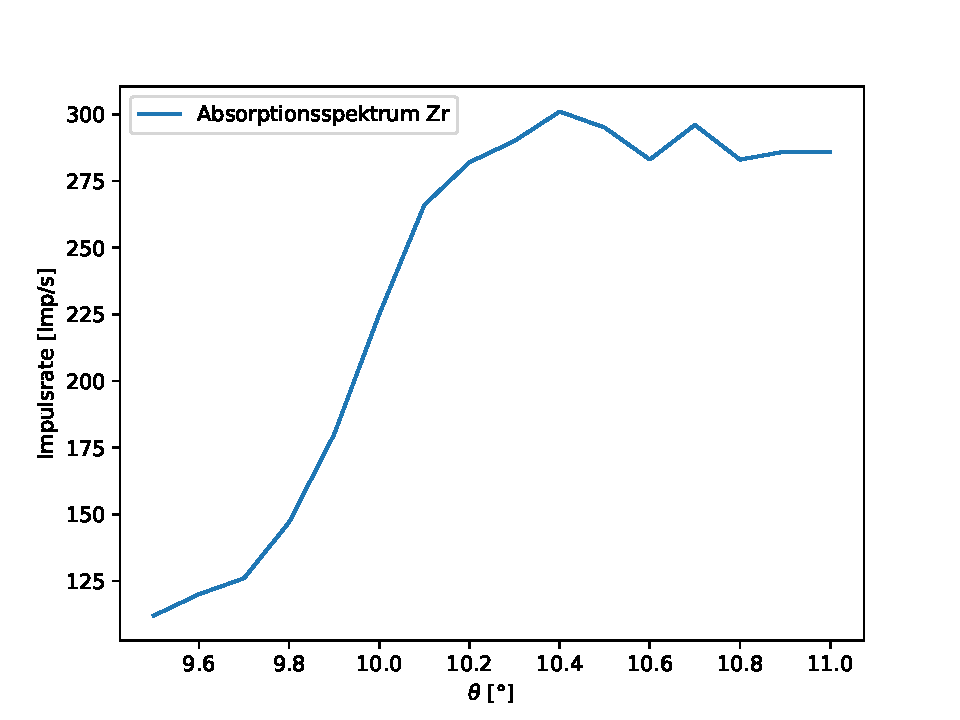
\includegraphics{Zirkonium.pdf}
              \caption{In der Abbildung ist das Absorptionsspektrum des Zirkonium-Absorbers aufgetragen.}
              \label{fig:Zirkonium}
            \end{figure}
            \FloatBarrier

           
            \newpage
            \section{Literaturverzeichnis}
                    [1] \textit{Versuchsanleitung V602 - Röntgenemission und -absorption.} TU Dortmund, 2020 \newline
                    [2] National Institute of Standards and Technology: \textit{Fundamental Physical Constants} 17.Mai.2020
                        \url{https://physics.nist.gov/cgi-bin/cuu/Value?r}
        
            \newpage

\end{document}
            



            
     